% !TEX encoding = UTF-8 Unicode
\documentclass[a4paper,12pt]{article}

\usepackage{mathptmx}
%\usepackage{tikz,pgfplots}
%\pgfplotsset{compat=newest}
%\usetikzlibrary{external}
%\tikzset{external/system call={latex \tikzexternalcheckshellescape -halt-on-error -interaction=batchmode -jobname "\image" "\texsource"; dvips -o "\image".eps "\image".dvi}}
%\usetikzlibrary{spy}
%\tikzexternalize
\usepackage{subfigure}
\usepackage[utf8]{inputenc} % Caracteres con acentos. 
\usepackage[spanish]{babel}
\usepackage{amsmath,delarray,amsthm} % enhances the typeset appearance of mathematical formulas\usepackage{graphicx}
\usepackage{graphicx} % Inclusión de gráficos. Soporte para \figura (más abajo) 
\usepackage{colortbl}
\usepackage{caption}
\usepackage[top=20mm,left=20mm,body={170mm,255mm}]{geometry}
\usepackage[colorlinks=true, urlcolor=blue]{hyperref}

\title{\large Método de Elementos Finitos\\
\bf Ejercicio sobre modelos de vigas y cálculo estático}
\author{José M.ª Goicolea, Nicola Tarque}
\date{27 nov 2022}
\begin{document}
\maketitle
\thispagestyle{empty}

Se considera un viaducto para ferrocarril de tablero continuo y recto, con cinco vanos de luces $L_{1}$ y $L_{5}= 33$ m, y $L_{2}$, $L_{3}$, y $L_{4}$ de $45$ m. La sección del tablero es del tipo cajón cuyas características son área $A=3.91\,\text{m}^{2}$, inercias según las direcciones locales (principales) $I_{1}=1.3921\,\text{m}^{4}$, $I_{2}=8.4693\,\text{m}^{4}$, módulo de torsión $J=2.675\,\text{m}^{4}$. 
Las propiedades mecánicas son módulo de elasticidad $E=3.20\,\text{GPa}$, coeficiente de Poisson $\nu=0.25$, constante de cortante $\kappa=5/6$. 

 
Se considera que el hormigón de la pila tiene las mismas propiedades mecánicas que el del tablero.



El apoyo intermedio es sobre una pila de altura $H_{1}=8\,\text{m}$ (aunque en un primer modelo se supondrá esta pila infinitamente rígida, es decir el tablero directamente apoyado en el punto intermedio). La figura siguiente presenta un croquis de la estructura.
\begin{figure}[h!]
	\subfigure[]{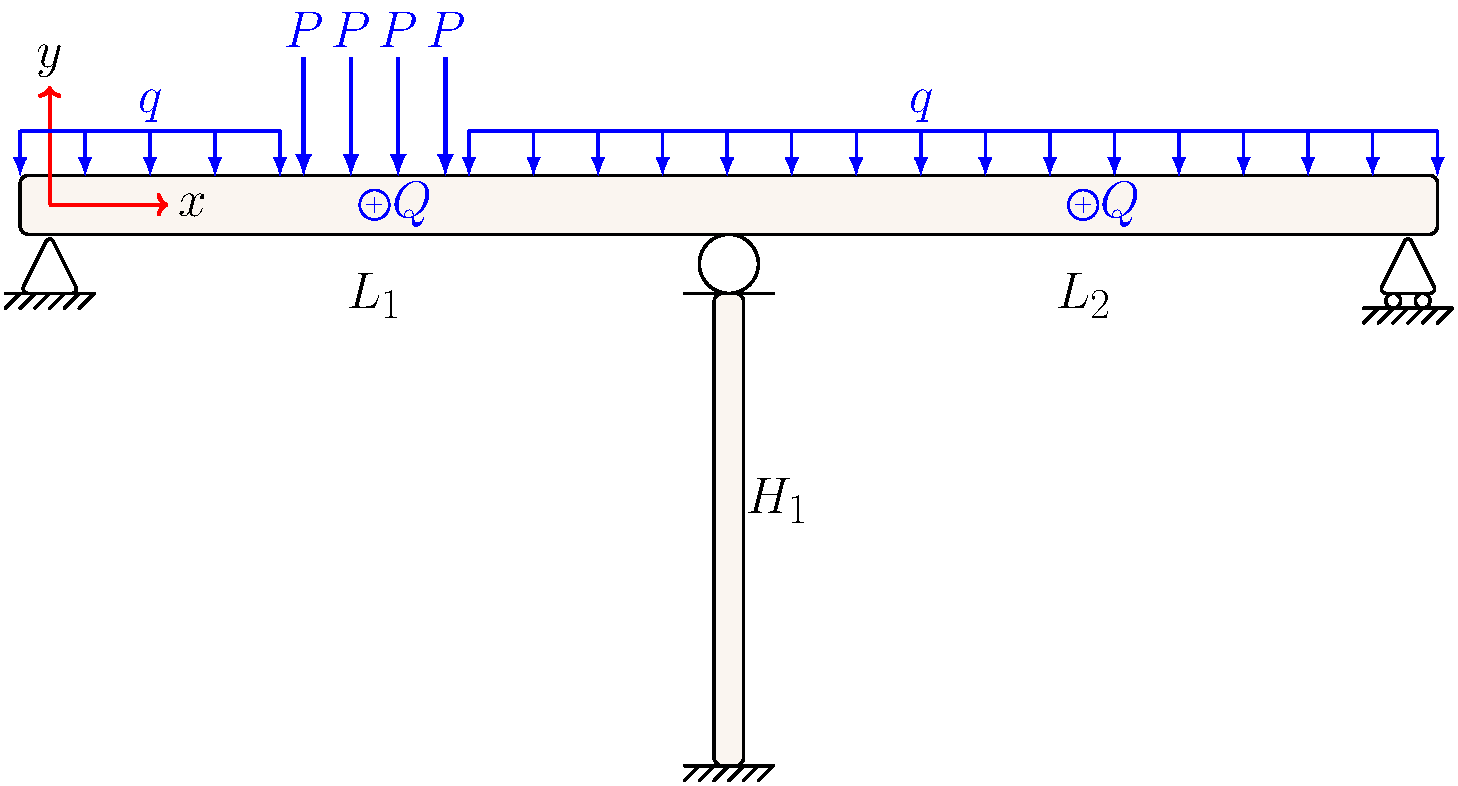
\includegraphics[width=0.70\textwidth]{figs/croquis}}%
	\subfigure[]{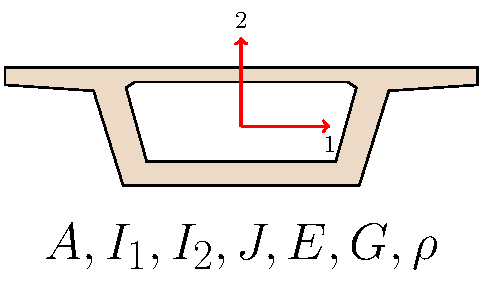
\includegraphics[width=0.30\textwidth]{figs/seccion}}
\end{figure}

La sección del tablero es de tipo cajón de hormigón pretensado, cuyas características son: área $A=3.91\,\text{m}^{2}$, inercias según las direcciones locales (principales) definidas arriba  $I_{1}=1.3921\,\text{m}^{4}$, $I_{2}=8.4693\,\text{m}^{4}$, módulo de torsión $J=2.675\,\text{m}^{4}$. 
Las propiedades mecánicas son: módulo de elasticidad $E=3.20\,\text{GPa}$, coeficiente de Poisson $\nu=0.25$, constante de cortante $\kappa=5/6$. 
La pila tiene siguientes características seccionales: area $A=2.5\,\text{m}^{2}$, inercias $I_{1}=1.302,~ I_{2}=0.208\,\text{m}^{4},\ J=0.6225\,\text{m}^{4}$. 
Se considera que el hormigón de la pila tiene las mismas propiedades mecánicas que el del tablero.

Se tomarán para el modelo unos ejes como se indica in la figura, con el origen en el extremo izquierdo, la dirección $x$ longitudinal al tablero, $y$ vertical y $z$ transversal a la estructura. 
El estribo izquierdo $x=0$ está fijo en todas las direcciones, mientras que el derecho tiene el movimiento longitudinal libre. El apoyo intermedio proporciona una restricción en las direcciones $y,z$, pero es deslizante en dirección longitudinal $x$ y permite este desplazamiento libremente al tablero. Los giros de torsión $\theta_{x}$ y transversales $\theta_{y}$ están impedidos en ambos estribos mientras que el de flexión vertical $\theta_{z}$ está libre.
El apoyo intermedio tiene unión perfecta para la torsión $\theta_{x}$ pero permite giros relativos del tablero en las componentes $\theta_{y}, \theta_{z}$.

Las cargas aplicadas sobre el puente son:
\begin{itemize}
 \item carga de peso propio
 \item carga de tren según el modelo LM71 como se indica en la figura, con las cargas puntuales verticales $P=250\,\text{kN}$ situadas en el primer vano, y la carga distribuida $q=80\,\text{kN/m}$ 
 \item cargas transversales en el medio de los dos vanos $Q=100\,\text{kN}$
\end{itemize}

El tablero se discretizará con $60$ elementos, la pila con $16$ elementos. Se proporcionan los siguientes modelos con elementos viga de 2 nodos, pequeñas deformaciones sin deformación a cortante:
\begin{itemize}
	\item Modelo 2D, en el plano $xy$, con apoyo en punto fijo (pila infinitamente rígida), sin considerar deformación por cortante. El fichero de input de FEAP es \href{http://stokes.mecanica.upm.es/MEFL_open/talleres/I2v2d-eb}{\texttt{I2v2d-eb}}.
%	\item Modelo 2D, en el plano $xy$, con apoyos en puntos fijos (pila infinitamente rígida), considerarando deformación por cortante. El fichero de input de FEAP es \textit{I2v2d-Timo}.
	\item Modelo 3D, incluyendo pila, sin considerar deformación por cortante. El fichero de input de FEAP es \href{http://stokes.mecanica.upm.es/MEFL_open/talleres/I2vp3d-eb}{\texttt{I2vp3d-eb}}.
%	\item Modelo 3D, incluyendo pila, considerando deformación por cortante. El fichero de input de FEAP es \textit{I2vp3d-Timo}.

\end{itemize}

Se pide:
\begin{itemize}
\item Ejecutar los cálculos con los modelos proporcionados. Determinar el desplazamiento vertical en el medio del segundo vano, la reacción vertical en el primer apoyo, el momento flector vertical en el centro del primer vano. Obtener gráficos del contorno de desplazamiento vertical y lateral.
\item Modificar las condiciones de contorno en los extremos del puente a empotrados (no hay no desplazamientos ni giros) y ejecutar los cálculos.
\item Crear modelos considerando deformación por cortante a partir de los modelos proporcionados y compara los desplazamientos verticales en los centros de vanos entre los modelos con y sin considerar la deformación por cortante.
\end{itemize}

\clearpage
\section*{Ejercicios propuestos}
\subsection*{Ejercicio propuesto 1}
Sea un puente isostático de un vano de 16 m de la luz. La sección del tablero es constante y de tipo cajón de hormigón pretensado, cuyas caráctristicas son: área $A=1.58$ m$^2$; inercias según las direcciones locales (principales) definidas arriba  $I_{1}=0.4987\,\text{m}^{4}$, $I_{2}=3.034\,\text{m}^{4}$, módulo de torsión $J=1.7067\,\text{m}^{4}$. 
Las propiedades mecánicas son: módulo de elasticidad $E=3.20\,\text{GPa}$,  coeficiente de Poisson $\nu=0.25$,  constante de cortante $\kappa=5/6$. 
Las cargas aplicadas sobre el puente son peso propio y 3 cargas puntuales ($P=250$ kN) situadas tal como se muestra en la siguiente figura:

\begin{figure}[h]
\centering
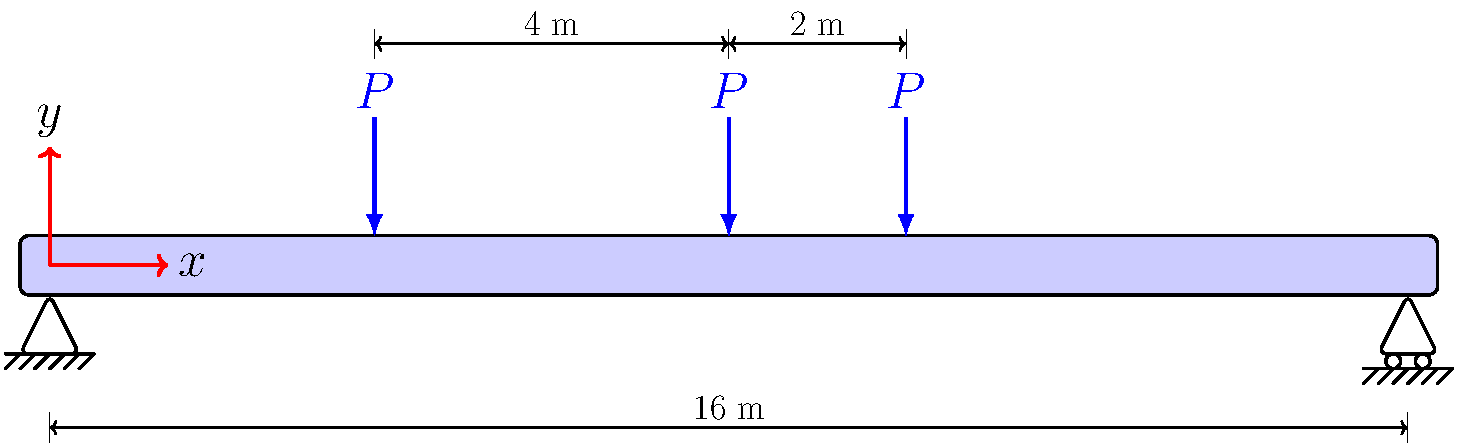
\includegraphics[width=0.8\textwidth]{figs/croquis1.pdf}
\label{fig.eje1}
\end{figure}

Se proporciona un modelo de FEAP que aún falta por definir las cargas aplicadas (descarga por este \href{http://stokes.mecanica.upm.es/MEFL_open/talleres/I1v2d-eb}{link}). Se pide:
\begin{itemize}
\item Completar el modelo y ejecutar el cálculo
\item Determinar el momento flector en el centro de vano y los giros en los dos apoyos
\end{itemize}

\clearpage

\subsection*{Ejercicio propuesto 2}
Sea un paso inferior de tipo pórtico rectangular de hormigón armado con una luz de 8.0 m. Se considera que el dintel tiene una sección transversal de $14.0\times1.0$ m y los muros hastiales tienen una de $14.0\times0.5$ m. Las propiedades mecánicas para el material de hormigón armado son módulo de elasticidad $E=3.20\,\text{GPa}$,  coeficiente de Poisson $\nu=0.25$,  constante de cortante $\kappa=5/6$. 
Las cargas aplicadas sobre el paso inferior son peso propio, cargas distribuidas ($q=80$ kN/m) y una carga longitudinal $Q=100$ kN como se muestra en la siguiente figura:
\begin{figure}[h]
\centering
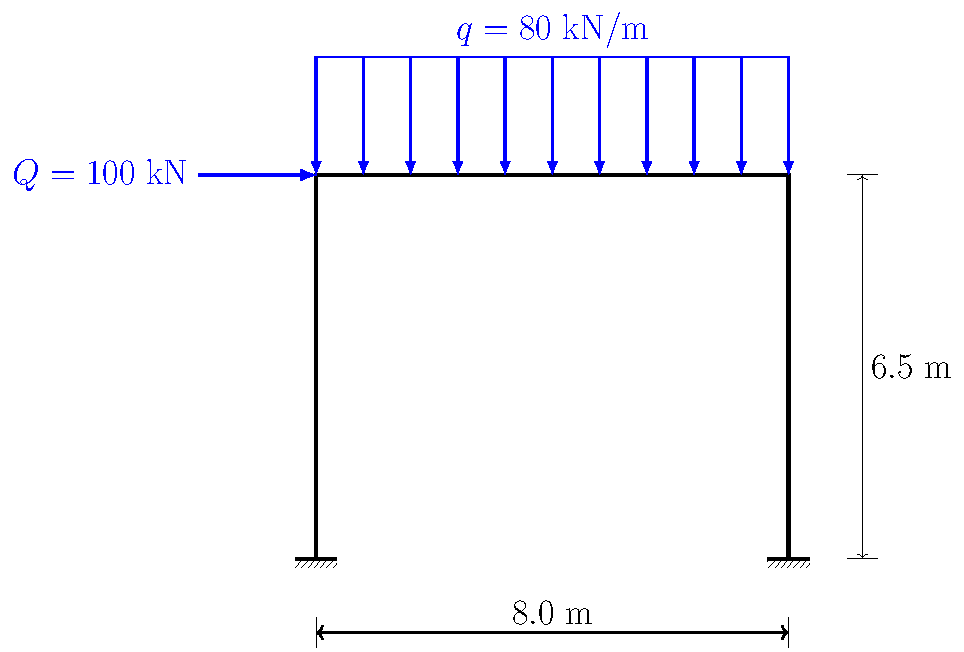
\includegraphics[width=0.7\textwidth]{figs/croquis2.pdf}
\end{figure}
Se considera que la cimentación está perfectamente empotrada. Se proporciona un modelo de FEAP, falta por definir los materiales y las cargas (se descarga con este \href{http://stokes.mecanica.upm.es/MEFL_open/talleres/Ip2d-eb}{link}). Se pide:

\begin{itemize}
\item Completar el modelo y ejecutar el cálculo
\item Determinar el momento flector y desplazamiento vertical en el centro de vano, desplazamiento horizontal en la esquina en la cual se aplica la carga horizontal, momento de reacción en las cimentaciones.
\end{itemize}

\end{document}
